\section{\Multidispatch{} Linearizability}
\label{sec:mdl}

In this section, we first define \multidispatch{} linearizability. 
We then show how applications built atop an \MDL{} system appear behave
identically (as far as users can tell) to the same application interacting
with a comparable \SDL{} system. Finally, we discuss existing implementations
of \SDL{} for single-shard systems. 

\subsection{Definition}
\label{sec:mdl:def}

\subsubsection{Failure Semantics}

We define \mdl failures as follows: a group of outstanding requests issued by a client will induce a prefix-closed set of success responses followed by a set of failed responses. It is possible that all of the requests succeed, and the set of failed responses will be empty. Importantly, if a request fails, all concurrent requests invoked by the same client with greater sequence numbers will also fail.

\subsection{External Equivalence}
\label{sec:mdl:equivalence}

\subsection{\MDL{} on One Shard}
\label{sec:mdl:single-shard}

In this section, we discuss Zookeeper and its implementation of \SDL{}.
We also show how such an approach does not extend to multiple shards.

\begin{figure}[!htb]
    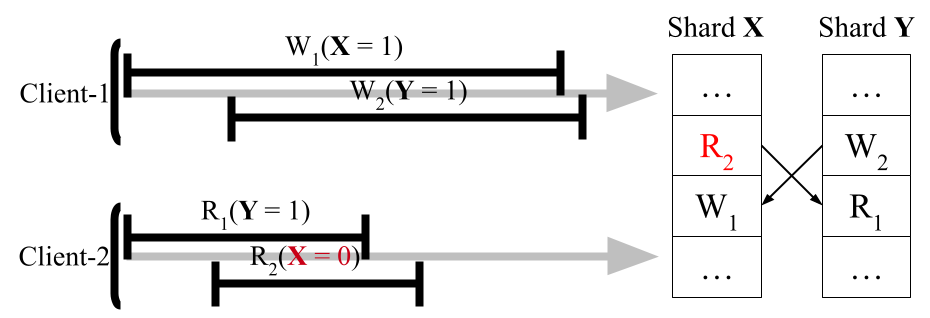
\includegraphics[scale=.45]{somet.png}
    \caption{Example execution where two concurrent clients each submit 2 concurrent requests. Assume keys \textbf{X} and \textbf{Y} are at different shards. It is possible that $R_2$ arrives before $W_1$ at shard \textbf{X}, and $W_2$ arrives before $R_1$ at shard \textbf{Y}. Since clients expect their concurrent requests to take affect in invocation order, if $R_1$ returns 1, then $W_1$ must have taken affect before $R_1$, so $R_2$ should necessarily return a value of 1.}
    \label{fig:concurrentbatches}
\end{figure}

For the single-shard setting, existing protocols come close to providing \MDL{}. A simple mechanism, such as per-client sequence numbers, can provide enough information for a shard leader to support invocation order for multiple requests from a single client. Such a solution does not suffice in the multi-shard setting, however, as shown in figure ~\ref{fig:concurrentbatches}. Linearizability is a local property, thus a single-shard protocol correctly scales to multiple shards. \MDL{}, however, is not a local property due to the possible interleaving of sets of concurrent requests across concurrent clients.
% Jeff: I don't think we want (or need) to make the claim below.
% This requires an \MDL{} protocol to use inter-shard communication in order to guarantee a safe total ordering that reflects issue order.

Sequence numbers are assigned at the client library 
and increase monotonically per shard. For example, a client issuing two requests for the first time to different keys that are on different shards will issue two requests both with sequence number 0. The shard leaders can then easily detect when a client's request
has arrived out of order and can buffer it until the necessary predecessor requests intended for the same shard arrive.